%!TEX root = practicum4.tex
The display method \t{display_circumscribed_circles}, see \autoref{lst:a:display_circumscribed_circles}, draws the Delaunay Triangulation and the circumscribed circles of three randomly chosen circles. To run the script \t{assignment4A} with this display method use the flag \t{circ}, the result of one such call is shown in \autoref{fig:b:circles}.

\lstinputlisting[linerange={157-158, 160-160, 168-168, 176-187}, label={lst:a:display_circumscribed_circles}, caption={The relevant part of the method \t{display_circumscribed_circles()}.}]{../assignment4a.py}

Circles are drawn with the provided method \t{draw_circle} which expects the centre and the radius of circle. The centre of the circle through all three points of a triangle is the circumcentre of the triangle, which is one of the results of \t{matplotlib.delaunay.delaunay()}. Since we have added the faces of the triangles in the same order as they were provided by the triangulation method the index of a face in \t{faces} attribute of the \t{DCEL} is the same as the index of its circumcentre in the \t{cens}. 

To determine the radius of a circle we compute the distance between one of the points on the circle, the vertices of the triangle, and its centre. We use the method \t{get_incident_face} on the \t{outer_component} of the face to get the vertices, see \autoref{lst:a:get_incident_face}

\lstinputlisting[linerange={51-60}, label={lst:a:get_incident_face}, caption={The method \t{get_incident_face()} in the class \t{HalfEdge}.}]{../halfedge.py}

\begin{figure}
	\centering
	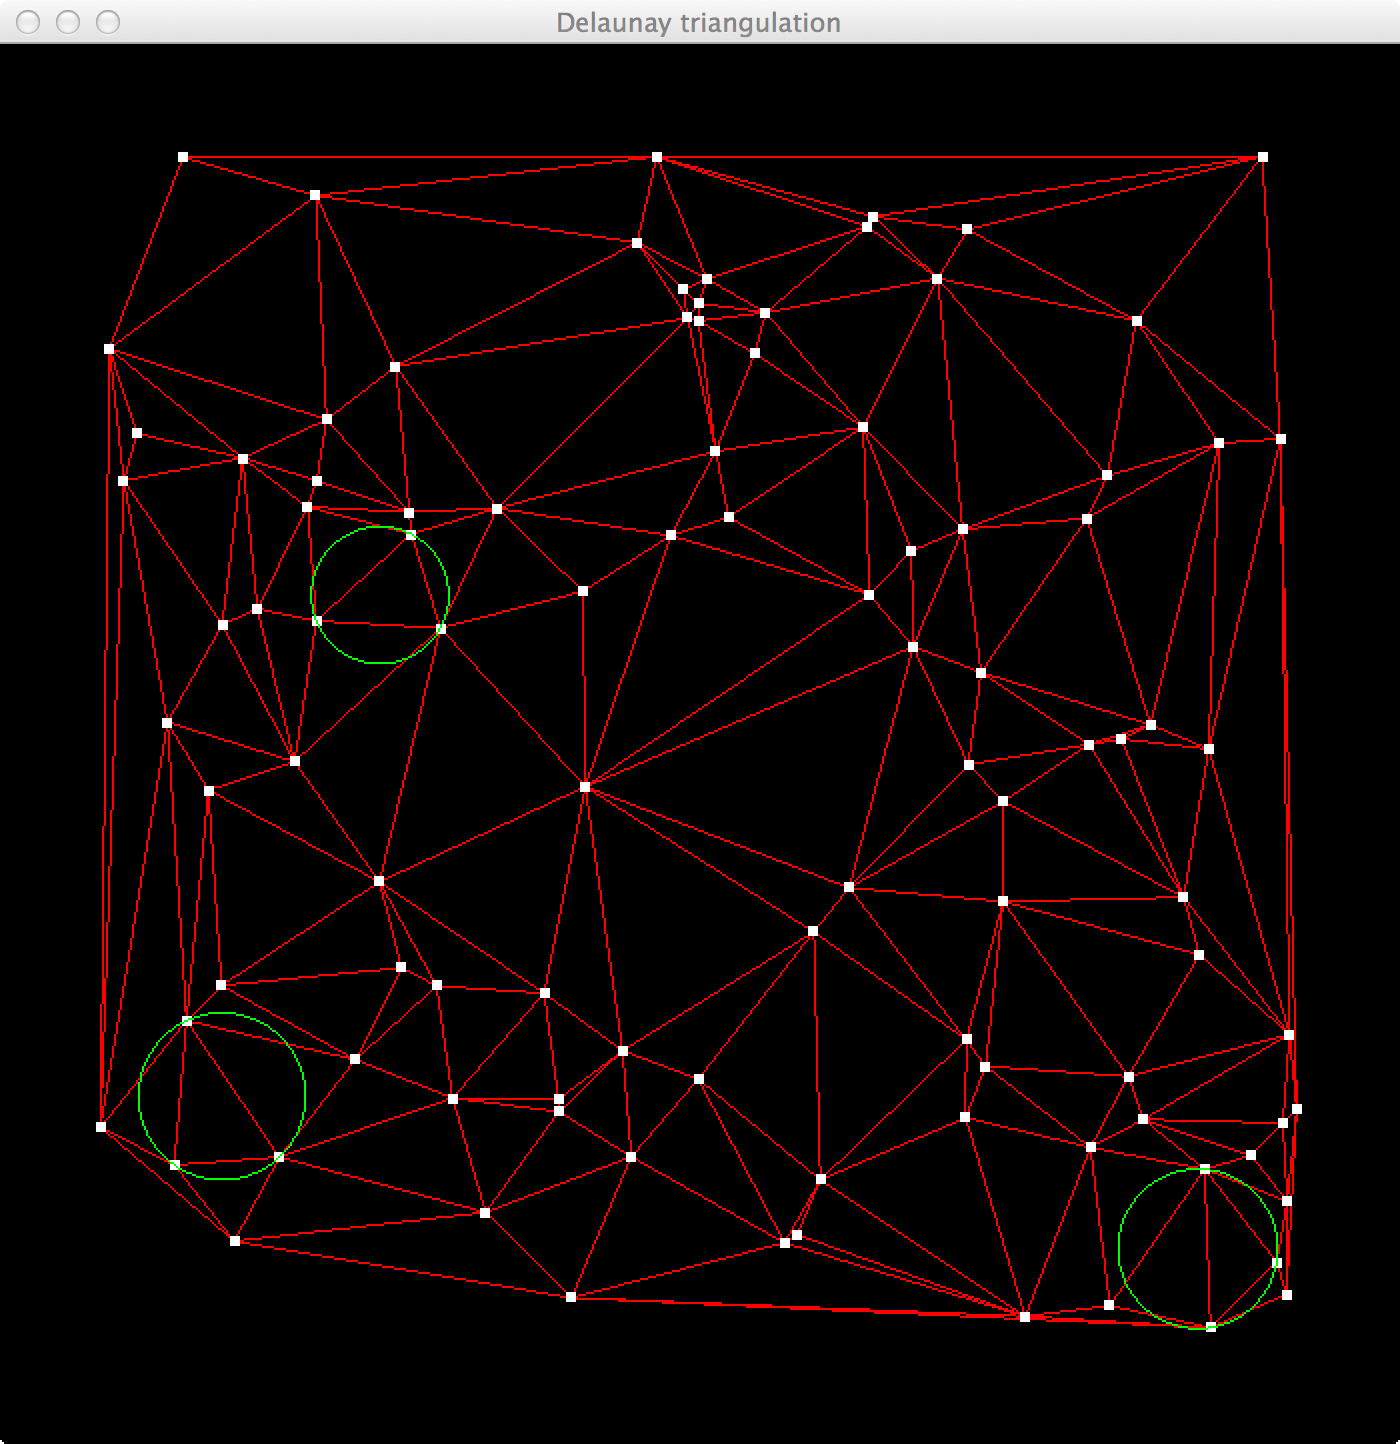
\includegraphics[width=0.405\textwidth]{./img/b_circles}
	\caption{The Delaunay triangulation of the white points is shown in red, the circumscribed circles of three randomly selected triangles is shown in green.}
	\label{fig:b:circles}
\end{figure}